\section{Physikalische Grundlagen}

\subsection{Helium-Neon-Laser}

\begin{figure}[H]
\begin{center}
  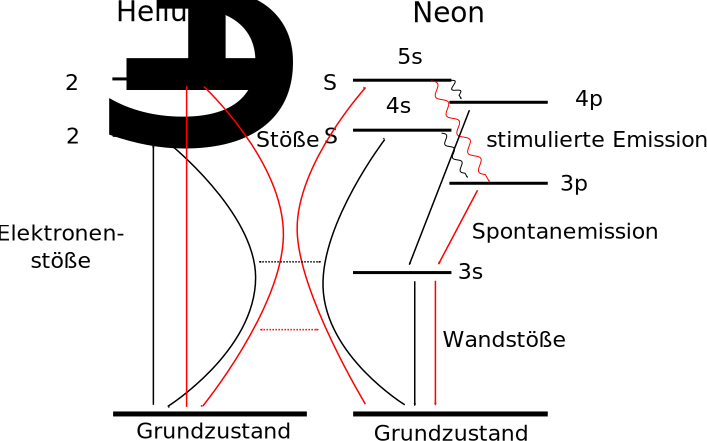
\includegraphics[width=0.8\textwidth]{../img/HeNe.pdf}
  \caption{Termschemata von Helium und Neon: Energieübergänge im Laser.
  In rot der Zyklus, der im Versuch verstärkt wird.}
  \label{img:HeNe}
\end{center}
\end{figure}

Ein Laser besteht aus drei Komponenten: Einer \emph{Pumpe},
die in einem \emph{aktiven Medium} Besetzungsinversion verursacht und \emph{Spiegeln},
die emittierte Strahlung zurück in das Medium reflektierten.
Die reflektierte Strahlung stimuliert im Medium Emission und verstärkt sich dadurch selbst.\\
Der im Versuch verwendete Laser ist ein Helium-Neon-Gaslaser.\footnote{
Die Ausführungen in diesem Abschnitt orientieren sich an \cite{dem3}.}
Der eigentliche Laserübergang findet beim Neon statt, das Helium dient nur zur Übertragung der Energie
auf das Neon:
Eine an der Röhre angelegte Spannung führt zu Gasentladung und Anregung der Heliumatome
in den metastabilen 2S-Zustand
(siehe \autoref{img:HeNe}).
Durch Stöße wird diese Energie auf Neonatome übertragen und diese in höhere s-Zustände angeregt.\\
Auf dem Rückweg in den Grundzustand können mehrere Übergänge als Laserübergänge verstärkt werden.
Am Versuchsaufbau wird durch geeignete Wahl der Spiegel
der Übergang 5s-3p verwendet, der eine Wellenlänge von 632.82\,nm besitzt.
Vom 3p-Zustand aus fallen die Neonatome schnell wieder spontan auf das 3s-Niveau und von dort aus
durch Wandstöße zurück in den Grundzustand.



\subsection{Der Mitführungskoeffizient als Konsequenz der speziellen Relativitätstheorie}

\subsubsection*{Relativistische Addition von Geschwindigkeiten}
Schon vor der Formulierung der speziellen Relativitätstheorie war durch verschiedene Experimente bekannt,
dass Strahlung von bewegten, optisch dichten Medien zum Teil mitgeführt wird.
Für die Geschwindigkeit $v$ der Strahlung im bewegten Medium mit Brechungsindex $n$, gemessen vom Ruhesystem,
gilt
\begin{equation}
\label{eq:mitf}
v = v' \pm \alpha \cdot w = \frac{c}{n} \pm \alpha \cdot w
\end{equation}
Die Geschwindigkeit des bewegten Systems ist $w$, $c$ die Lichtgeschwindigkeit,
$v'$ die Lichtgeschwindigkeit im bewegten System und
$\alpha$ der Mitführungskoeffizient.
Das Auftreten des Mitführungskoeffizienten wurde damals mit einer teilweisen Mitführung des Äthers erklärt.\\
In der Relativitätstheorie folgt der Mitführungskoeffizient als Grenzfall für kleine Geschwindigkeiten
aus der Formel für die Geschwindigkeitsaddition bei Transformation in bewegte Inertialsysteme:
\begin{equation}
\label{}
v=\frac{v'+w}{1+\frac{v' \cdot w}{c^2}}
\end{equation}
Division des Bruchs durch $c$ liefert
\begin{equation}
\label{}
v=\frac{\frac{v'}{c}+\frac{w}{c}}{\frac{1}{c}+\frac{v' \cdot \frac{w}{c}}{c^2}}
\end{equation} 
und aus der Taylorentwicklung für $w \ll c$, also $w/c \ll 1$, folgt
\begin{equation}
\label{}
v \approx v' + (c-\frac{v'^2}{c})\cdot \frac{w}{c}+ (-v'+\frac{v'^3}{c^2})\cdot \left(\frac{w}{c}\right)^2
\end{equation}
Da für die Lichtgeschwindigkeit $v'$ im Medium mit Brechungsindex $n$ gilt
\begin{equation}
\label{}
v'=\frac{c}{n}
\end{equation}
lautet die Taylorentwicklung bis zum linearen Term
\begin{equation}
\label{}
v \approx v' + (1-\frac{1}{n^2})\cdot w
\end{equation}
Dies entspricht dem Zusammenhang, den A. J. \textsc{Fresnel} aus der Äthertheorie ableitete.

\subsubsection*{Relativistischer Dopplereffekt}
Die Relativitätstheorie liefert aber noch einen weiteren Beitrag zum Mitführungskoeffizienten.
Der relativistische Dopplereffekt, der die Frequenzveränderung einer E/M-Welle
bei einer Relativbewegung zwischen Sender und Empfänger beschreibt,
führt zur Aufnahme eines weiteren Terms in die Gleichung für den Koeffizienten.
Die Frequenz des empfangenen Signals $f_\text{E}$ beiträgt bei der Senderfrequenz $f_\text{S}$
\begin{equation}
\label{}
f_\text{E} = f_\text{S} \cdot \sqrt{\frac{c \pm w}{c \mp w}}
\end{equation}
Der Mitführungskoeffizient unter Berücksichtigung des Dopplereffekts lautet (Herleitung siehe \cite{staatsex})
\begin{equation}
\label{eq:alpha:theo}
\alpha = 1 - \frac{1}{n^2} - \frac{\lambda}{n} \cdot \frac{\Delta n}{\Delta \lambda}
\end{equation}
$\lambda$ ist die Wellenlänge des Lichts und $\Delta n / \Delta \lambda$ die lineare Dispersion im Medium.

\subsection{Bestimmung des Mitführungskoeffizienten mit dem Ringlaser}
Die Herleitung der Formel für die Bestimmung des Mitführungskoeffizienten mit dem vorliegenden Aufbau erfordert
aufwändige geometrische Überlegungen und findet sich in \cite{staatsex}.
Hier werden nur kurz die Grundzüge der Herleitung dargelegt.\\
Die optische Gesamtlänge des Resonators $L$ ist die Summe des Produkts aller Teilstreckenlängen $l_i$ mit dem 
jeweiligen Brechungsindex $n_i$
\begin{equation}
\label{}
L = \sum_i{l_i \cdot n_i}
\end{equation}
Für den Laser gilt die Randbedingung, dass eine ganze Zahl $N$ von Wellenzügen mit der Wellenlänge $\lambda$
in $L$ liegen muss:
\begin{equation}
\label{}
L = N \cdot \lambda
\end{equation}
Für die Bestimmung des Mitführungskoeffizienten ist die Änderung der optischen Gesamtlänge $\Delta L$ interessant.
Diese Änderung wird nur durch die Änderung des effektiven Brechungsindex $n_\text{Q}$
in der rotierenden Quarzscheibe
verursacht. Für die optische Länge $L_\text{Q}$ des Quarz mit der Dicke $l_\text{Q}$ gilt
\begin{equation}
\label{}
L_\text{Q} = n_\text{Q} \cdot l_\text{Q} \refeq{eq:mitf} \frac{c}{\frac{c}{n_\text{Q}} \pm \alpha \cdot w}
\end{equation}
Wenn man davon ausgeht, dass eine kleine Änderung der opt. Länge $\Delta L$ die Anzahl $N$ der Wellenzüge
im Resonator nicht ändert, so gilt
\begin{equation}
\label{}
\frac{\Delta L}{L} = \frac{\Delta \lambda}{\lambda}
\end{equation}
Es wird also eine Änderung $\Delta \lambda$ der Wellenlänge des Laserlichts verursacht,
die für eine Strahlkomponente positiv, für die andere negativ ist.
Dieser kleine Unterschied der Wellenlängen führt zur Ausbildung einer Schwebung mit der Frequenz
$\Delta \nu$, die mit der Photodiode gemessen werden kann.
Der Mitführungskoeffizient $\alpha$ kann dann mit folgendem Zusammenhang bestimmt werden:
\begin{equation}
\label{eq:alpha:exp}
\alpha = \frac{L \cdot \lambda \cdot \Delta \nu}{2 \cdot n_\text{Q} \cdot \omega \cdot d \cdot x_0}
\end{equation}
$\omega$, $d$ und $x_0$ sind Größen am Versuchsaufbau, die in \autoref{sec:aufbau} erklärt werden.


